\documentclass[fleqn]{article}
\usepackage[nodisplayskipstretch]{setspace}
\usepackage{amsmath, nccmath, bm}
\usepackage{amssymb}
\usepackage{enumitem}
\usepackage{etoolbox}
\usepackage[normalem]{ulem}
\usepackage[hidelinks,colorlinks=true,urlcolor=blue,linkcolor=black]{hyperref}
\usepackage{graphicx}
\usepackage{float}
\usepackage{changepage}
\usepackage{environ,capt-of}
\usepackage{matlab-prettifier}

\makeatletter
\begingroup
  \catcode`\$=6 %
  \catcode`\#=12 %
  \gdef\href@split$1#$2#$3\\$4{%
    \hyper@@link{$1}{$2}{\uline{$4}}% or \underline
    \endgroup
  }%
\endgroup

\let\oldfigure\figure% Store original figure float environment
\let\endoldfigure\endfigure
\RenewEnviron{figure}[1][H]{% Update figure environment
  %\par\vspace{\intextsep}% Assume in-text placement, so insert appropriate vertical spacing
  \noindent
  % \patchcmd{<cmd>}{<search>}{<replace>}{<success>}{<failure>}
  \patchcmd{\BODY}{\caption}{\captionof{figure}}{}{}% Replace \caption with \captionof{figure} inside \BODY
  % Set "figure"
  \begin{minipage}{\linewidth}
    \BODY
  \end{minipage}
  %\par\vspace{\intextsep}% Assume in-text placement, so insert appropriate vertical spacing
}

\newcommand{\zerodisplayskip}{
	\setlength{\abovedisplayskip}{0pt}%
	\setlength{\belowdisplayskip}{0pt}%
	\setlength{\abovedisplayshortskip}{0pt}%
	\setlength{\belowdisplayshortskip}{0pt}%
	\setlength{\mathindent}{0pt}}
	
\newcommand{\norm}[1]{\left \lVert #1 \right \rVert}
	
\title{Homework 2}
\author{Owen Sowatzke}
\date{February 21, 2024}

\begin{document}

	\offinterlineskip
	\setlength{\lineskip}{12pt}
	\zerodisplayskip
	\maketitle
	
	\begin{enumerate}
		\item  The nearest neighbor method is used with the following labeled training data in a two class, two feature problem. Show clearly the decision boundaries obtained. Indicate all break points and slopes correctly
		
		Class 1 = $\{(0,0)^T,\:(0,1)^T\}$
		
		Class 2 = $\{(1,0)^T,\:(0,0.5)^T\}$
		
		Consider the distance between an input sample $\mathbf{x}$ and two training samples $\mathbf{x_1}$ and $\mathbf{x_2}$. By comparing the distances from the input sample to each training sample, we can determine which training sample the input is closest to. The boundary condition occurs when the input sample is equidistant from each training sample. 
		
		\begin{equation*}
			\norm{\mathbf{x} - \mathbf{x_2}} \overset{\omega_1}{\underset{\omega_2}{\gtrless}} \norm{\mathbf{x} - \mathbf{x_1}} \Rightarrow \norm{\mathbf{x} - \mathbf{x_2}}^2  \overset{\omega_1}{\underset{\omega_2}{\gtrless}} \norm{\mathbf{x} - \mathbf{x_1}}^2
		\end{equation*}
		
		\begin{equation*}
			(\mathbf{x} - \mathbf{x_2})^T(\mathbf{x} - \mathbf{x_2}) \overset{\omega_1}{\underset{\omega_2}{\gtrless}} (\mathbf{x} - \mathbf{x_1})^T(\mathbf{x} - \mathbf{x_1})
		\end{equation*}
		
		\begin{equation*}
			\norm{\mathbf{x}}^2 - \mathbf{x_2}^T\mathbf{x} - \mathbf{x}^T\mathbf{x_2} + \norm{\mathbf{x_2}}^2 \overset{\omega_1}{\underset{\omega_2}{\gtrless}} \norm{\mathbf{x}}^2 - \mathbf{x_1}^T\mathbf{x} - \mathbf{x}^T\mathbf{x_1} + \norm{\mathbf{x_1}}^2
		\end{equation*}
		
		\begin{equation*}
			- \mathbf{x_2}^T\mathbf{x} - \mathbf{x}^T\mathbf{x_2} + \norm{\mathbf{x_2}}^2 \overset{\omega_1}{\underset{\omega_2}{\gtrless}} - \mathbf{x_1}^T\mathbf{x} - \mathbf{x}^T\mathbf{x_1} + \norm{\mathbf{x_1}}^2
		\end{equation*}
		
		\begin{equation*}
			- (\mathbf{x_2}^T\mathbf{x})^T - \mathbf{x}^T\mathbf{x_2} + \norm{\mathbf{x_2}}^2 \overset{\omega_1}{\underset{\omega_2}{\gtrless}} - (\mathbf{x_1}^T\mathbf{x})^T - \mathbf{x}^T\mathbf{x_1} + \norm{\mathbf{x_1}}^2
		\end{equation*}
		
		\begin{equation*}
			- \mathbf{x}^T\mathbf{x_2} - \mathbf{x}^T\mathbf{x_2} + \norm{\mathbf{x_2}}^2 \overset{\omega_1}{\underset{\omega_2}{\gtrless}} - \mathbf{x}^T\mathbf{x_1} - \mathbf{x}^T\mathbf{x_1} + \norm{\mathbf{x_1}}^2
		\end{equation*}
		
		\begin{equation*}
			- 2\mathbf{x}^T\mathbf{x_2} + \norm{\mathbf{x_2}}^2 \overset{\omega_1}{\underset{\omega_2}{\gtrless}} - 2\mathbf{x}^T\mathbf{x_1} + \norm{\mathbf{x_1}}^2
		\end{equation*}
		
		\begin{equation*}
			2\mathbf{x}^T\mathbf{x_1} - 2\mathbf{x}^T\mathbf{x_2} - \norm{\mathbf{x_1}}^2 + \norm{\mathbf{x_2}}^2 \overset{\omega_1}{\underset{\omega_2}{\gtrless}} 0
		\end{equation*}
		
		\begin{equation*}
			2\mathbf{x}^T(\mathbf{x_1} - \mathbf{x_2}) - \norm{\mathbf{x_1}}^2 + \norm{\mathbf{x_2}}^2 \overset{\omega_1}{\underset{\omega_2}{\gtrless}} 0
		\end{equation*}
		
		We start by finding the boundary conditions between the first sample of class 1 and the samples of class 2.
		
		Boundary between $(0,0)^T$ and $(1,0)^T$:
		
		\begin{equation*}
			2 \begin{bmatrix} x & y \end{bmatrix} \begin{bmatrix}-1\\ 0\end{bmatrix} - 0 + 1 \overset{\omega_1}{\underset{\omega_2}{\gtrless}} 0 \Rightarrow -2x + 1 \overset{\omega_1}{\underset{\omega_2}{\gtrless}} 0 \Rightarrow 2x \overset{\omega_2}{\underset{\omega_1}{\gtrless}} 1 \Rightarrow x \overset{\omega_2}{\underset{\omega_1}{\gtrless}} 0.5			
		\end{equation*}
		
		Boundary between $(0,0)^T$ and $(0,0.5)^T$:
		
		\begin{equation*}
			2 \begin{bmatrix} x & y \end{bmatrix} \begin{bmatrix}0\\ -0.5\end{bmatrix} - 0 + 0.25 \overset{\omega_1}{\underset{\omega_2}{\gtrless}} 0 \Rightarrow -y + 0.25 \overset{\omega_1}{\underset{\omega_2}{\gtrless}} 0 \Rightarrow y \overset{\omega_2}{\underset{\omega_1}{\gtrless}} 0.25		
		\end{equation*}
		
		$\therefore$ we are closer to sample $(0,0)^T$ if $y < 0.25$ and $x < 0.5$.
		
		Next, find the boundary conditions between the second sample of class 1 and the samples of class 2.
		
		Boundary between $(0,1)^T$ and $(1,0)^T$:
		
		\begin{equation*}
			2 \begin{bmatrix} x & y \end{bmatrix} \begin{bmatrix}-1\\ 1\end{bmatrix} - 1 + 1 \overset{\omega_1}{\underset{\omega_2}{\gtrless}} 0 \Rightarrow -2x + 2y \overset{\omega_1}{\underset{\omega_2}{\gtrless}} 0 \Rightarrow 2y \overset{\omega_1}{\underset{\omega_2}{\gtrless}} 2x \Rightarrow y \overset{\omega_1}{\underset{\omega_2}{\gtrless}} x		
		\end{equation*}
		
		Boundary between $(0,1)^T$ and $(0,0.5)^T$:
		
		\begin{equation*}
			2 \begin{bmatrix} x & y \end{bmatrix} \begin{bmatrix}0\\ 0.5\end{bmatrix} - 1 + 0.25 \overset{\omega_1}{\underset{\omega_2}{\gtrless}} 0 \Rightarrow y - 0.75 \overset{\omega_1}{\underset{\omega_2}{\gtrless}} 0 \Rightarrow y \overset{\omega_1}{\underset{\omega_2}{\gtrless}} 0.75		
		\end{equation*}
		
		$\therefore$ we are closer to sample $(0,1)^T$ if $y > 0.75$ and $y > x$.
		
		If we take the union between the two regions, we can determine the boundary conditions between class 1 and class 2.
		
		After taking the union of these regions, we find that we should choose class 1 if $y < 0.25$ and $x < 0.5$ or if $y > 0.75$ and $y > x$. 
		
		\item In a two class problem using two features, we have the following four training vectors:
		
		Class $\omega_1 = [(0,0)^T\quad(1,0)^T]$
		
		Class $\omega_2 = [(0,1)^T\quad(1,1)^T]$
		
		Use the perceptron criterion method with $\rho_k = 1$ to determine the solution vector $\mathbf{w}$. Use an all zero vector as the starting point for $\mathbf{w}$. Show the $\mathbf{w}$ vector after each iteration.
		
		To start, we need to determine the $\mathbf{\hat{x}}$ vectors. For samples in class $\omega_1$, $\mathbf{\hat{x}}$ is given as follows:
		
		\begin{equation*}
			\mathbf{\hat{x}} = \begin{bmatrix}\mathbf{x}\\ 1 \end{bmatrix}
		\end{equation*}
			
		For samples in class $\omega_2$, $\mathbf{\hat{x}}$ is given as follows:
		
		\begin{equation*}
			\mathbf{\hat{x}} = \begin{bmatrix} -\mathbf{x}\\ -1 \end{bmatrix}
		\end{equation*}
		
		$\therefore$ the $\mathbf{\hat{x}}$ vectors are given as follows:
		
		\begin{equation*}
			\mathbf{\hat{x}_1} = \begin{bmatrix} 0 \\ 0 \\ 1 \end{bmatrix} \quad \mathbf{\hat{x}_2} = \begin{bmatrix} 1 \\ 0 \\ 1 \end{bmatrix} \quad \mathbf{\hat{x}_3} = \begin{bmatrix} 0 \\ -1 \\ -1 \end{bmatrix} \quad \mathbf{\hat{x}_4} = \begin{bmatrix} -1 \\ -1 \\ -1 \end{bmatrix}
		\end{equation*}		
		
		For each iteration, define the set of misclassified samples as follows:
		
		\begin{equation*}
			E = \{\mathbf{\hat{x}}: \mathbf{w}^T\mathbf{\hat{x}} \leq 0\}
		\end{equation*}
		
		After each iteration, we can then update the $\mathbf{w}$ vector as follows:
		
		\begin{equation*}
			\mathbf{w}^{(n+1)} = \mathbf{w}^{(n)} + \rho_k\sum_{\mathbf{\hat{x}} \in E}{\mathbf{\hat{x}}}
		\end{equation*}
		
		We contain this process until all samples are correctly classified (i.e. $\mathbf{w}$ vector does not change).
		
		Iteration 1:
		
		\begin{equation*}
			\mathbf{w}^T\mathbf{\hat{x}_1} = 0 \quad \mathbf{w}^T\mathbf{\hat{x}_2} = 0 \quad \mathbf{w}^T\mathbf{\hat{x}_3} = 0 \quad \mathbf{w}^T\mathbf{\hat{x}_4} = 0
		\end{equation*}
		
		$\Rightarrow \mathbf{\hat{x}_1}, \mathbf{\hat{x}_2}, \mathbf{\hat{x}_3}, \mathbf{\hat{x}_4} \in E$.
		
		\begin{equation*}
			\mathbf{w}^{(1)} = \mathbf{w}^{(0)} + \rho_k\sum_{\mathbf{\hat{x}} \in E}{\mathbf{\hat{x}}}
		\end{equation*}
			
		\begin{equation*}
			= \begin{bmatrix} 0 \\ 0 \\ 0 \end{bmatrix}			 + \left(\begin{bmatrix}0\\0\\1\end{bmatrix} + \begin{bmatrix}1\\0\\1\end{bmatrix} + \begin{bmatrix}0\\-1\\-1\end{bmatrix} + \begin{bmatrix}-1\\-1\\-1\end{bmatrix}\right) = \begin{bmatrix}0\\-2\\0\end{bmatrix}
		\end{equation*}
		
		Iteration 2:
		
		\begin{equation*}
			\mathbf{w}^T\mathbf{\hat{x}_1} = 0 \quad \mathbf{w}^T\mathbf{\hat{x}_2} = 0 \quad \mathbf{w}^T\mathbf{\hat{x}_3} = 2 \quad \mathbf{w}^T\mathbf{\hat{x}_4} = 2
		\end{equation*}
		
		$\Rightarrow \mathbf{\hat{x}_1}, \mathbf{\hat{x}_2} \in E$.
		
		\begin{equation*}
			\mathbf{w}^{(2)} = \mathbf{w}^{(1)} + \rho_k\sum_{\mathbf{\hat{x}} \in E}{\mathbf{\hat{x}}}
		\end{equation*}
			
		\begin{equation*}
			= \begin{bmatrix} 0 \\ -2 \\ 0 \end{bmatrix}			 + \left(\begin{bmatrix}0\\0\\1\end{bmatrix} + \begin{bmatrix}1\\0\\1\end{bmatrix}\right) = \begin{bmatrix}1\\-2\\2\end{bmatrix}
		\end{equation*}
		
		Iteration 3:
		
		\begin{equation*}
			\mathbf{w}^T\mathbf{\hat{x}_1} = 2 \quad \mathbf{w}^T\mathbf{\hat{x}_2} = 3 \quad \mathbf{w}^T\mathbf{\hat{x}_3} = 0 \quad \mathbf{w}^T\mathbf{\hat{x}_4} = -1
		\end{equation*}
		
		$\Rightarrow \mathbf{\hat{x}_3}, \mathbf{\hat{x}_4} \in E$.
		
		\begin{equation*}
			\mathbf{w}^{(3)} = \mathbf{w}^{(2)} + \rho_k\sum_{\mathbf{\hat{x}} \in E}{\mathbf{\hat{x}}}
		\end{equation*}
			
		\begin{equation*}
			= \begin{bmatrix} 1 \\ -2 \\ 2 \end{bmatrix}			 + \left(\begin{bmatrix}0\\-1\\-1\end{bmatrix} + \begin{bmatrix}-1\\-1\\-1\end{bmatrix}\right) = \begin{bmatrix}0\\-4\\0\end{bmatrix}
		\end{equation*}
		
		Iteration 4:
		
		\begin{equation*}
			\mathbf{w}^T\mathbf{\hat{x}_1} = 0 \quad \mathbf{w}^T\mathbf{\hat{x}_2} = 0 \quad \mathbf{w}^T\mathbf{\hat{x}_3} = 4 \quad \mathbf{w}^T\mathbf{\hat{x}_4} = 4
		\end{equation*}
		
		$\Rightarrow \mathbf{\hat{x}_1}, \mathbf{\hat{x}_2} \in E$.
		
		\begin{equation*}
			\mathbf{w}^{(4)} = \mathbf{w}^{(3)} + \rho_k\sum_{\mathbf{\hat{x}} \in E}{\mathbf{\hat{x}}}
		\end{equation*}
			
		\begin{equation*}
			= \begin{bmatrix} 0 \\ -4 \\ 0 \end{bmatrix}			 + \left(\begin{bmatrix}0\\0\\1\end{bmatrix} + \begin{bmatrix}1\\0\\1\end{bmatrix}\right) = \begin{bmatrix}1\\-4\\2\end{bmatrix}
		\end{equation*}
		
		Iteration 5:
		
		\begin{equation*}
			\mathbf{w}^T\mathbf{\hat{x}_1} = 2 \quad \mathbf{w}^T\mathbf{\hat{x}_2} = 3 \quad \mathbf{w}^T\mathbf{\hat{x}_3} = 2 \quad \mathbf{w}^T\mathbf{\hat{x}_4} = 1
		\end{equation*}
		
		$\Rightarrow E = \{\emptyset\}$
		
		$\therefore$ all samples are correctly classified and the final value of $\mathbf{w}$ is given by:
		
		\begin{equation*}
			\mathbf{w} = \begin{bmatrix}1 \\ -4 \\ 2\end{bmatrix}
		\end{equation*}
		
		\item Consider the following training data:
		
		Class $\omega_1 = [(0,0)^T\quad(1,0)^T\quad(0,-1)^T]$
		
		Class $\omega_2 = [(0,1)^T\quad(1,2)^T\quad(-1,0)^T]$
		
		Determine the MSE vector $\mathbf{w}$ if $\mathbf{b} = [1\:1\:1\:1\:1\:1]^T$. Use the generalized inverse to find the solution vector. Is the data linearly separable?
		
		For each sample of training data $\mathbf{x}$. Define the vector $\mathbf{\hat{x}}$ as follows:
		
		\begin{equation*}
			\mathbf{\hat{x}} = \begin{bmatrix} \mathbf{x} \\ 1 \end{bmatrix}			
		\end{equation*}
		
		For each sample $\mathbf{x}$ contained in class $\omega_2$, we need to multiply the vector $\mathbf{\hat{x}}$ by $-1$. After performing this multiplication, the definition for $\mathbf{\hat{x}}$  for samples in class $\omega_2$ is given by:
		
		\begin{equation*}
			\mathbf{\hat{x}} = \begin{bmatrix} -\mathbf{x} \\ -1 \end{bmatrix}			
		\end{equation*}
		
		We can then form the matrix $\mathbf{A}$ from the vectors $\mathbf{\hat{x}_i}$:
		
		\begin{equation*}
			\mathbf{A} = \begin{bmatrix} \mathbf{\hat{x}_1}^T \\ \vdots \\ \mathbf{\hat{x}_n}^T \end{bmatrix}					
		\end{equation*}
		
		The generalized inverse of $\mathbf{A}$ is then defined as:
		
		\begin{equation*}
			\mathbf{A}^{\dag} = (\mathbf{A^T}\mathbf{A})^{-1}\mathbf{A}^T
		\end{equation*}
		
		Using the generalized inverse $\mathbf{A}^{\dag}$, we can find the MSE vector $\mathbf{w}$.
		
		\begin{equation*}
			\mathbf{w} = \mathbf{A}^{\dag}\mathbf{b}
		\end{equation*}
			
		For the provided training data, we first need to solve for the matrix $\mathbf{A}$. Doing so results in the following:
		
		\begin{equation*}
			\mathbf{A} = \begin{bmatrix}
				0  &  0 &  1 \\
				1  &  0 &  1 \\
				0  & -1 &  1 \\
				0  & -1 & -1 \\
			   -1  & -2 & -1 \\
			    1  &  0 & -1
			\end{bmatrix}
		\end{equation*}
		
		Next, using the formula given above, we can solve for the generalized inverse $\mathbf{A}^{\dag}$, the result of this operation is given below:
		
		\begin{equation*}
			\mathbf{A}^{\dag} = \begin{bmatrix} 
			   -0.0270 &  0.4054 &  0.1081 &  0.1622 & -0.1351 &  0.4595 \\
			   -0.0541 & -0.1892 & -0.2838 & -0.1757 & -0.2703 & -0.0811 \\
			    0.1892 &  0.1622 &  0.2432 & -0.1351 & -0.0541 & -0.2162
			\end{bmatrix}
		\end{equation*}
		
		Finally, we can solve for the vector $\mathbf{w}$ as follows:
		
		\begin{equation*}
			\mathbf{w} = \mathbf{A}^{\dag}\mathbf{b} = \begin{bmatrix} 0.9730 \\ -1.0541 \\ 0.1892 \end{bmatrix}
		\end{equation*}
		
		The data is linearly separable if $\mathbf{A}\mathbf{w} > \mathbf{0}$
		
		\begin{equation*}
			\mathbf{A}\mathbf{w} = \begin{bmatrix}
				0.1892 \\
    				1.1622 \\
   	 			1.2432 \\
    				0.8649 \\
    				0.9459 \\
    				0.7838
			\end{bmatrix} > \mathbf{0}
		\end{equation*}
		
		$\therefore$, the data is linearly separable.
		
		\item Compute Exercise:
		
		Using the IRIS data set available at \href{https://en.wikipedia.org/wiki/IRIS_flower_data_set}{https://en.wikipedia.org/wiki/\\IRIS\_flower\_data\_set}, design a 1-nearest neighbor classifier. Then, test each sample using the 1-NN rule to determine its class, and compare it to its true label. Tabulate your results in the form of a confusion table.
		
		Because the IRIS data set for this problem was small, I used leave-one-out cross-validation (LOOCV) to generate the confusion table. Specifically, for each training sample, I designed a 1-nearest neighbor classifier by leaving out the selected sample and training with the rest of the data. Then, I classified the selected sample using the generated classifier. Finally, I tabulated the classification results for each training sample in a confusion matrix. The software I wrote to perform these operations is given in Appendix \ref{nearest_neighbor} and attached with the submission. The resulting confusion matrix is given in Figure \ref{1nn_confusion_matrix}.
		
		\begin{figure}[H]				
			\centerline{\fbox{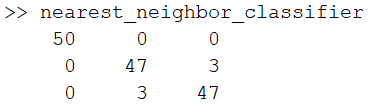
\includegraphics[width=0.5\textwidth]{1nn_confusion_matrix.png}}}
			\caption{Confusion Matrix Output by 1-Nearest Neighbor Classifier.}
			\label{1nn_confusion_matrix}
		\end{figure}
		
		\pagebreak
		
		\item Computer Exercise:
		
		Using the IRIS data set, design a Fisher LDF that discriminates between the Setosa (class 1), and the other two classes (Versicolor and Verginica combined together as class 2). What is the overall classification accuracy? Tabulate your results in the form of a confusion matrix.
		
		In my software, I computed Fisher's Linear Discriminant ($\mathbf{w}$) using the following formula:
		
		\begin{equation*}
			\mathbf{w} = \mathbf{S_w}^{-1}(\mathbf{m_1} - \mathbf{m_2})
		\end{equation*}
		
		where $\mathbf{m_1}$ was the mean of the class 1 data, $\mathbf{m_2}$ was the mean of the class 2 data, and $\mathbf{S_w}$ was defined as follows:
		
		\begin{equation*}
			\mathbf{S_w} = \mathbf{S_1} + \mathbf{S_2}
		\end{equation*}
		
		In the above formula, $\mathbf{S_1}$ and $\mathbf{S_2}$ represent the covariance of the class 1 and class 2 data respectively. 
		
		Once I had the linear discriminant, I projected the data onto it. Next to classify the data, I assumed that the projected data of each class had a Guassian distribution. This assumption allowed me to classify the data using the following minimum mean-squared error classifier:
		
		\begin{equation*}
			\frac{(x - \mu_2)^2}{2\sigma_2^2} - \frac{(x - \mu_1)^2}{2\sigma_1^2} \overset{\omega_1}{\underset{\omega_2}{\gtrless}} \text{ln}\left[\frac{P(\omega_2)}{P(\omega_1)}\cdot\frac{\sigma_1}{\sigma_2}\right]
		\end{equation*}
		
		I derived the means and variances in the above formula from the projected data and assumed equal prior probabilities for both classes. 
		
		Using this classifier on the projected data, I was able to generate a confusion matrix and determine the classification accuracy. My code for this problem is included in Appendix \ref{fisher_ldf} and attached with the submission. To visualize the classification, I also generated a histogram of the projected data and plotting the resulting decision boundaries. This histogram is given in Figure \ref{fisher_ldf_histogram}.
		
		\begin{figure}[H]				
			\centerline{\fbox{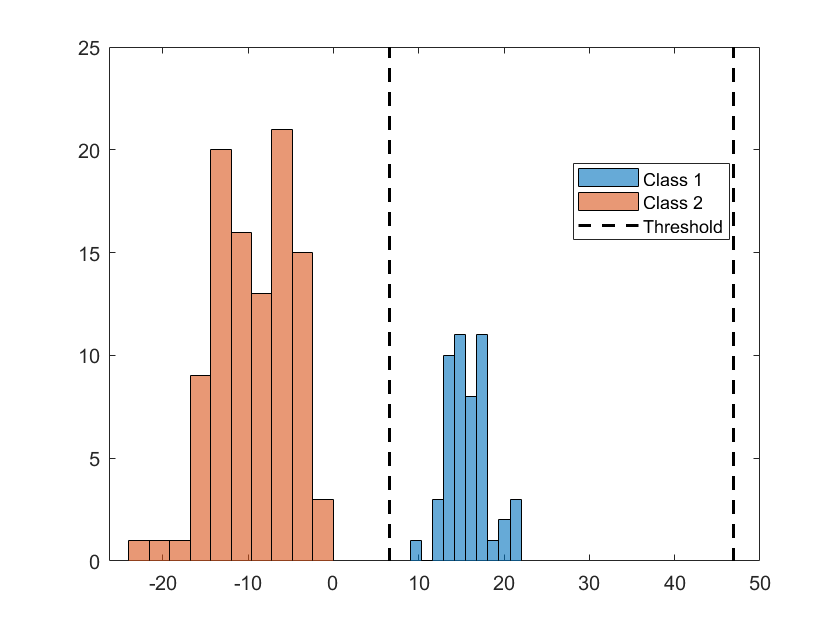
\includegraphics[width=0.9\textwidth]{fisher_ldf_histogram.png}}}
			\caption{Histogram of Data Projected onto Fisher's Linear Discriminant.}
			\label{fisher_ldf_histogram}
		\end{figure}
		
		Finally, the confusion matrix and classification accuracy, output by my program, are given in Figure \ref{fisher_ldf_stats} below.
		
		\begin{figure}[H]				
			\centerline{\fbox{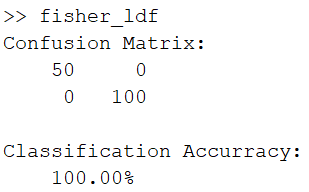
\includegraphics[width=0.5\textwidth]{fisher_ldf_stats.png}}}
			\caption{Output of Fisher Linear Discriminant Function}
			\label{fisher_ldf_stats}
		\end{figure}
	\end{enumerate}
	
	\pagebreak
	\appendix
	\section{Nearest Neighbor Classifier}
	\label{nearest_neighbor}
	\lstset{style=Matlab-editor,basicstyle=\ttfamily\footnotesize}
	\lstinputlisting{nearest_neighbor_classifier.m}
	\raggedbottom
	\pagebreak
	\section{Fisher's Linear Discriminant}
	\label{fisher_ldf}
	\lstset{style=Matlab-editor,basicstyle=\ttfamily\footnotesize}
	\lstinputlisting{fisher_ldf.m}
	\raggedbottom
\end{document}